\documentclass[11pt]{article}

%%%%%%%%%%%%
% Packages %
%%%%%%%%%%%%
\hyphenpenalty=10000
\usepackage{tocloft}
\renewcommand\cftsecleader{\cftdotfill{\cftdotsep}}
\usepackage{xcolor}
\usepackage{empheq}
\usepackage{hyperref}
\usepackage{epstopdf}
\usepackage{braket}
\usepackage{upgreek}
\usepackage{caption}
\usepackage{booktabs}
\usepackage{subcaption}
\usepackage{amssymb,latexsym,amsmath,gensymb}
\usepackage{latexsym}
\usepackage{graphicx}
\usepackage{float}
\usepackage{enumitem}
\usepackage{pdflscape}
\usepackage{url}
\usepackage{tikz, calc}
\usetikzlibrary{shapes.geometric, arrows, calc}
\tikzstyle{norm} = [rectangle, rounded corners, minimum width=2cm, minimum height=1cm,text centered, draw=black]
\tikzstyle{arrow} = [thick, ->, >=stealth]

\providecommand{\e}[1]{\ensuremath{\times 10^{#1}}} 
\providecommand{\mb}[1]{\mathbf{#1}}
\providecommand{\mh}[1]{\mathbf{\hat{#1}}}
\providecommand{\bs}[1]{\boldsymbol{#1}} 
\providecommand{\intinf}{\int_{-\infty}^{\infty}}
\providecommand{\fig}[4]{
  % filename, width, caption, label
\begin{figure}[h]
 \captionsetup{width=1.0\linewidth}
 \centering
 \includegraphics[width = #2\textwidth]{#1}
 \caption{#3}
 \label{fig:#4}
\end{figure}
}

\newcommand{\tensor}[1]{\overset{\text{\tiny$\leftrightarrow$}}{\mb{#1}}}
\newcommand{\tunderbrace}[2]{\underbrace{#1}_{\textstyle#2}}
\providecommand{\figs}[7]{
  % filename1, filename2, caption1, caption2, label1, label2, shift
\begin{figure}[H]
\centering
\begin{minipage}[b]{.45\textwidth}
  \centering
  \includegraphics[width=1.0\linewidth]{#1}
  \captionsetup{justification=justified, singlelinecheck=true}
  \caption{#3}
  \label{fig:#5}
\end{minipage}
\hspace{2em}
\begin{minipage}[b]{.45\textwidth}
  \centering
  \includegraphics[width=1.0\linewidth]{#2}
  \vspace{#7em}
  \captionsetup{justification=justified}
  \caption{#4}
  \label{fig:#6}
\end{minipage}
\end{figure}
}
\makeatletter

\providecommand{\code}[1]{
\begin{center}
\lstinputlisting{#1}
\end{center}
}
\setlength{\parindent}{0pt}
%%%%%%%%%%%
% Spacing %
%%%%%%%%%%%
% Margins
\usepackage[
top    = 1.5cm,
bottom = 1.5cm,
left   = 1.5cm,
right  = 1.5cm]{geometry}

% Indents, paragraph space
\usepackage{parskip} 

% Section spacing
\usepackage{titlesec}
\titlespacing*{\title}
{0pt}{0ex}{0ex}
\titlespacing*{\section}
{0pt}{0ex}{0ex}
\titlespacing*{\subsection}
{0pt}{0ex}{0ex}
\titlespacing*{\subsubsection}
{0pt}{0ex}{0ex}

% Line spacing
\linespread{1.1}

%%%%%%%%%%%%
% Document %
%%%%%%%%%%%%
\begin{document}
\title{\vspace{-2.5em} Relating Spherical Coordinates In Rotated Frames\vspace{-1em}} \author{Talon Chandler}% and Patrick La Rivi\`ere}
\date{\vspace{-1em}June 9, 2017\vspace{-1em}}
\maketitle

\section{Introduction}
In these notes we will relate typical spherical coordinates (Figure
\ref{fig:frames_a}) to obliquely rotated (Figure \ref{fig:frames_b}) and
orthogonal (Figure \ref{fig:frames_c}) spherical coordinates.
\begin{figure*}[h]
 \captionsetup{width=1.0\linewidth}
 \centering
 \begin{subfigure}[t]{0.33\textwidth}
   \centering
   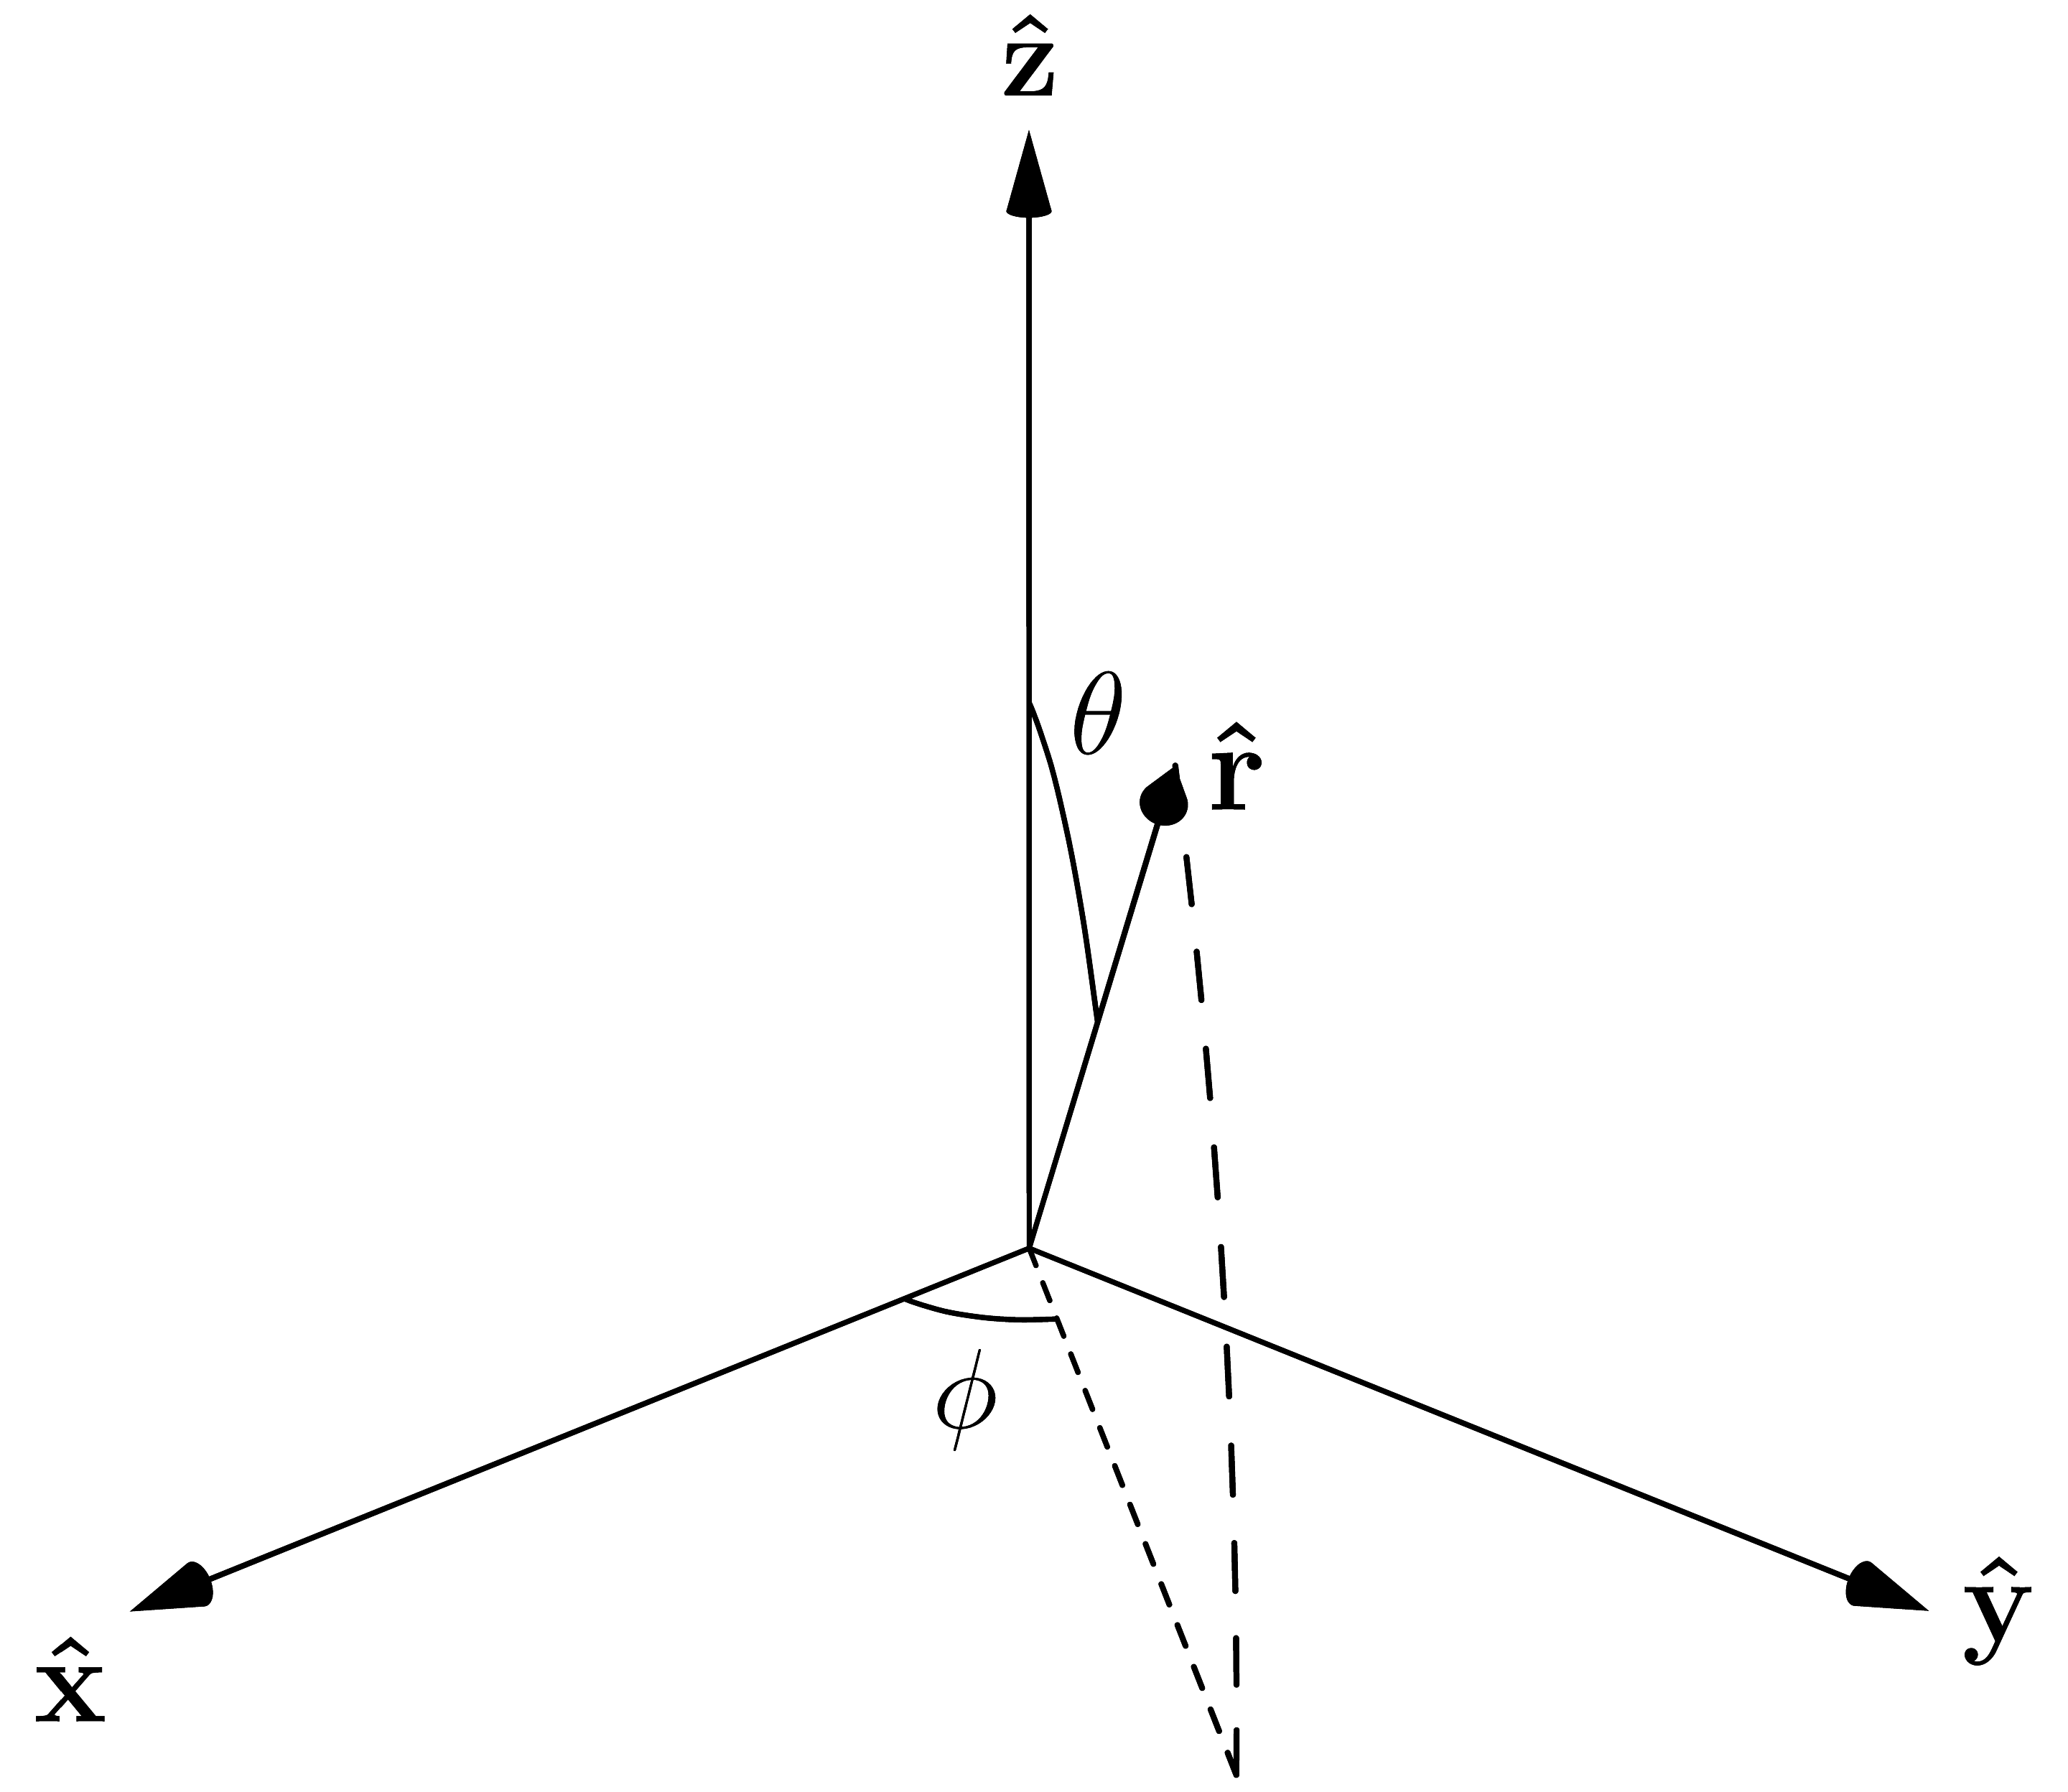
\includegraphics[width = 1.0\textwidth]{../figures/frame_a.pdf}
   \caption{Typical spherical coordinates}
   \label{fig:frames_a}
 \end{subfigure}%
 ~
 \begin{subfigure}[t]{0.33\textwidth}
   \centering
   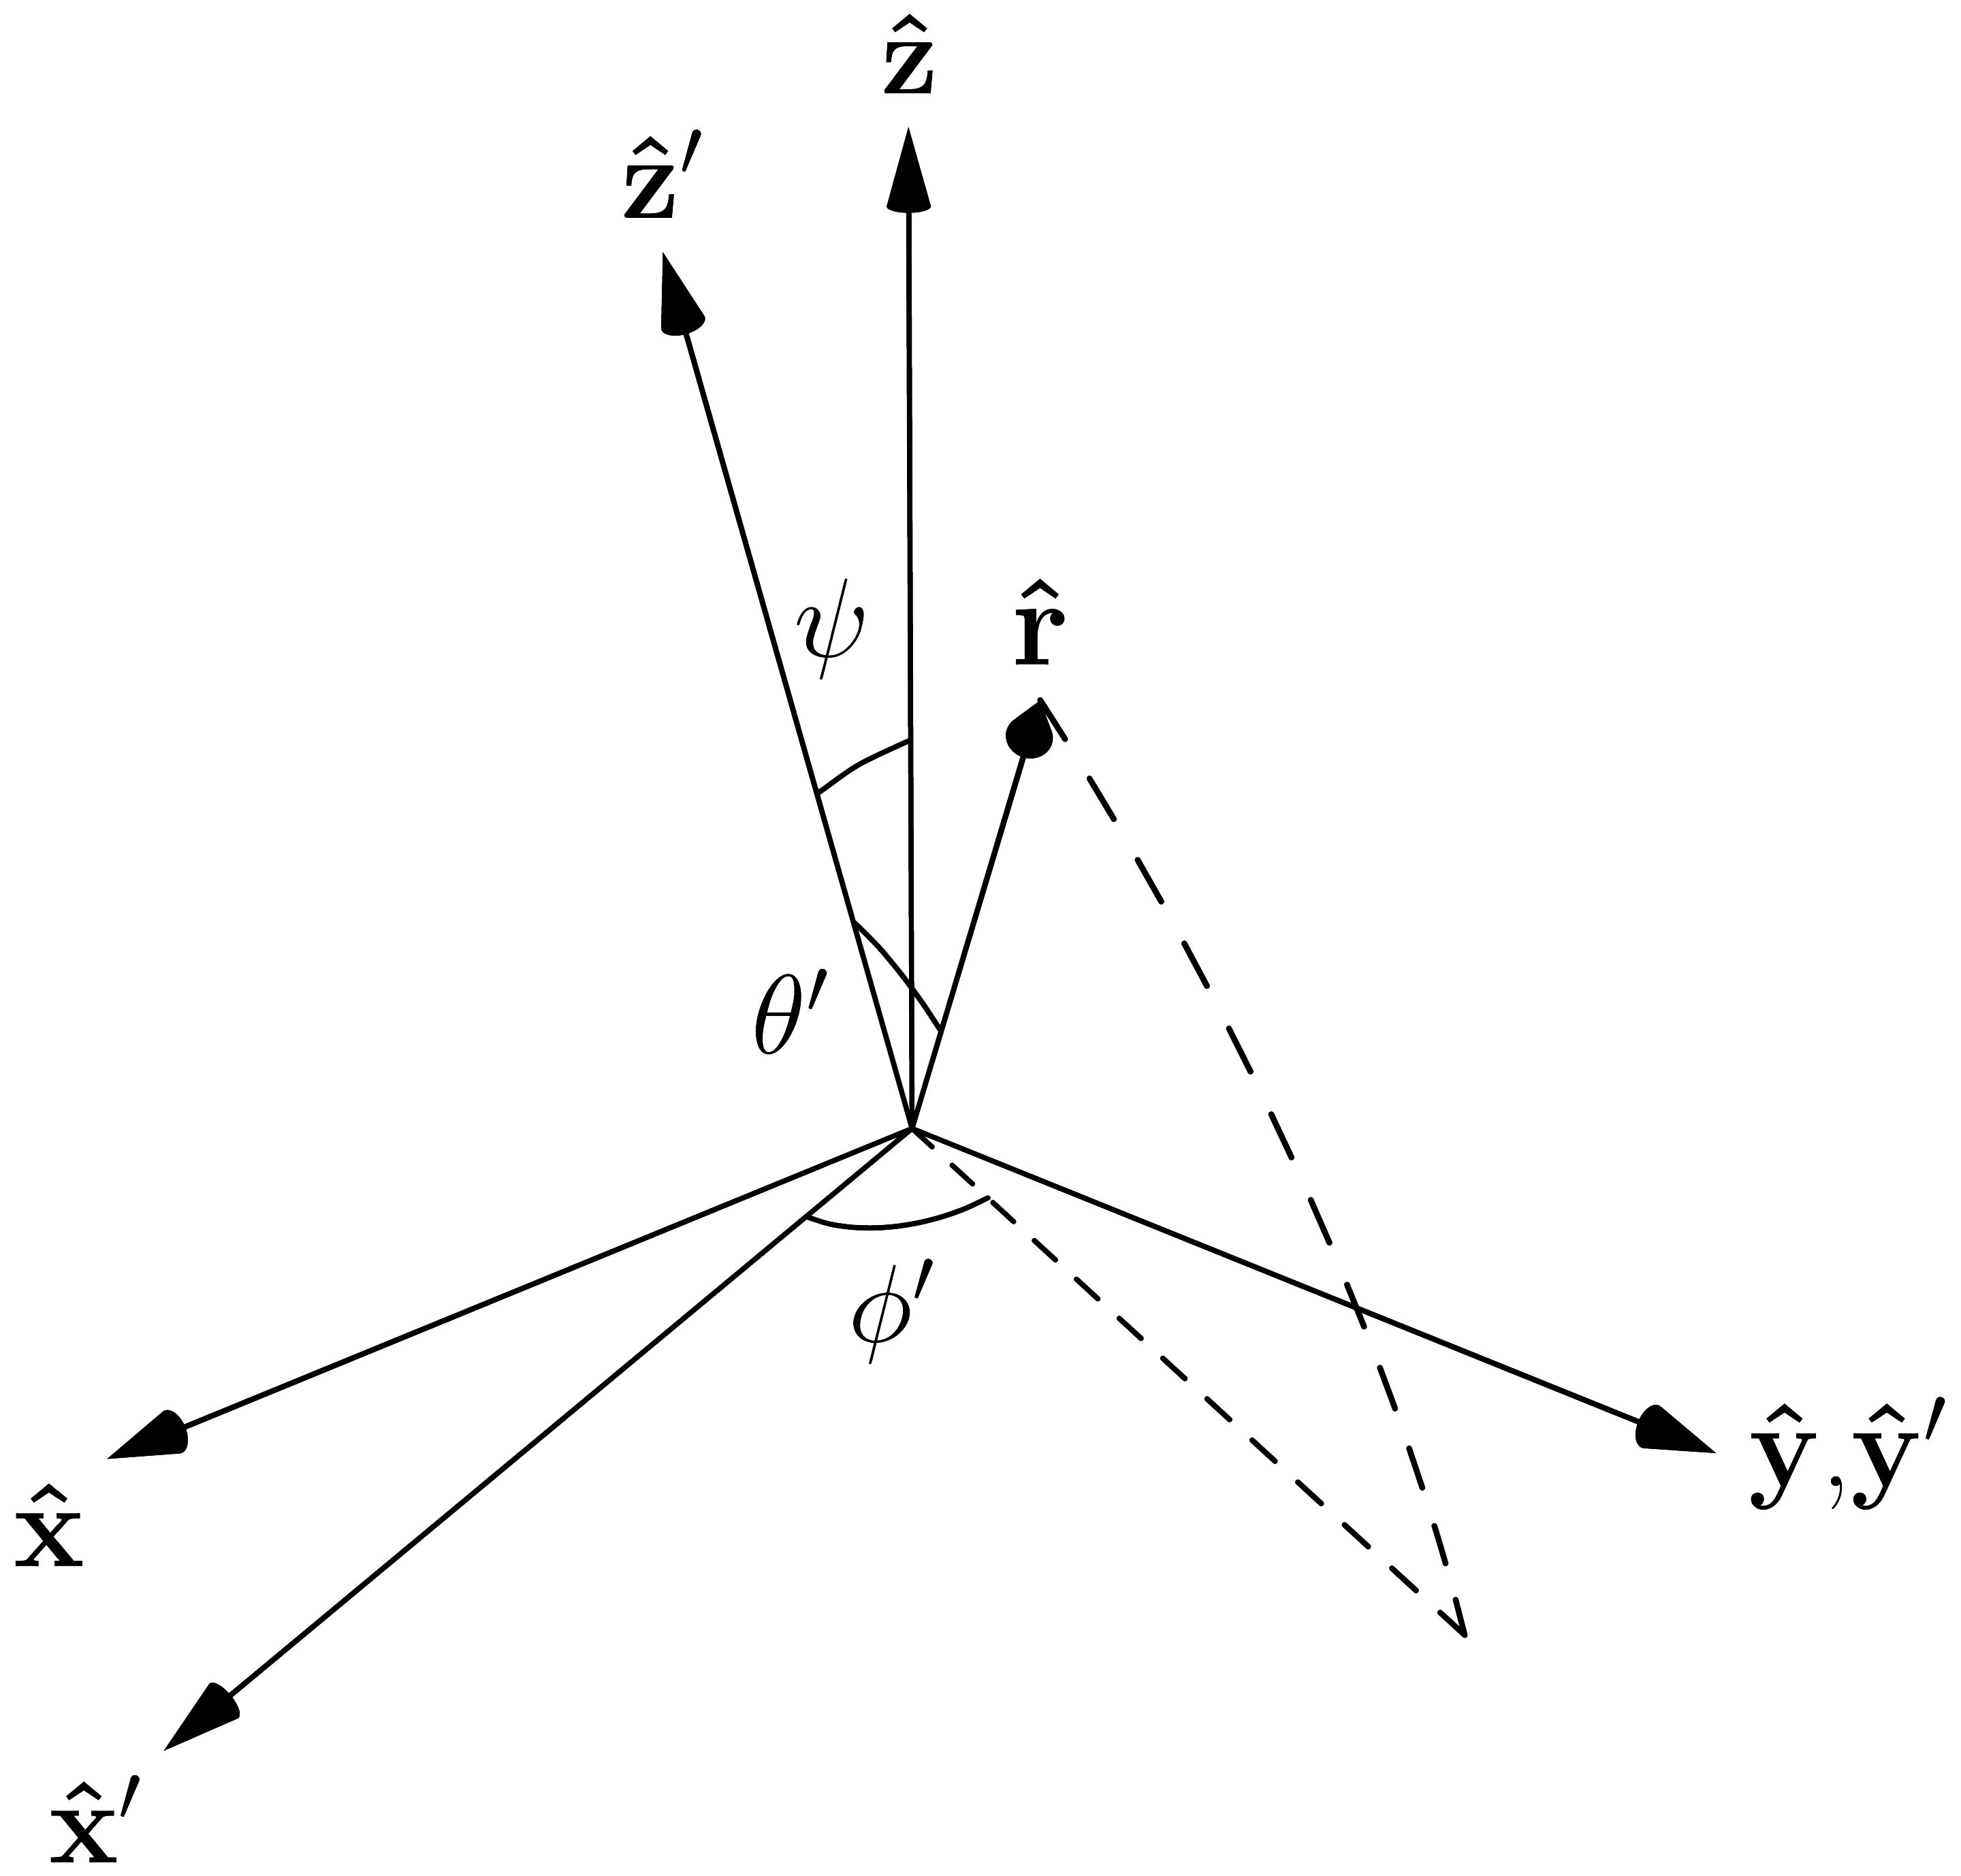
\includegraphics[width = 1.0\textwidth]{../figures/frame_b.pdf}
   \caption{$\psi$-rotated spherical coordinates}
   \label{fig:frames_b}
 \end{subfigure}%
 ~
 \begin{subfigure}[t]{0.33\textwidth}
   \centering
   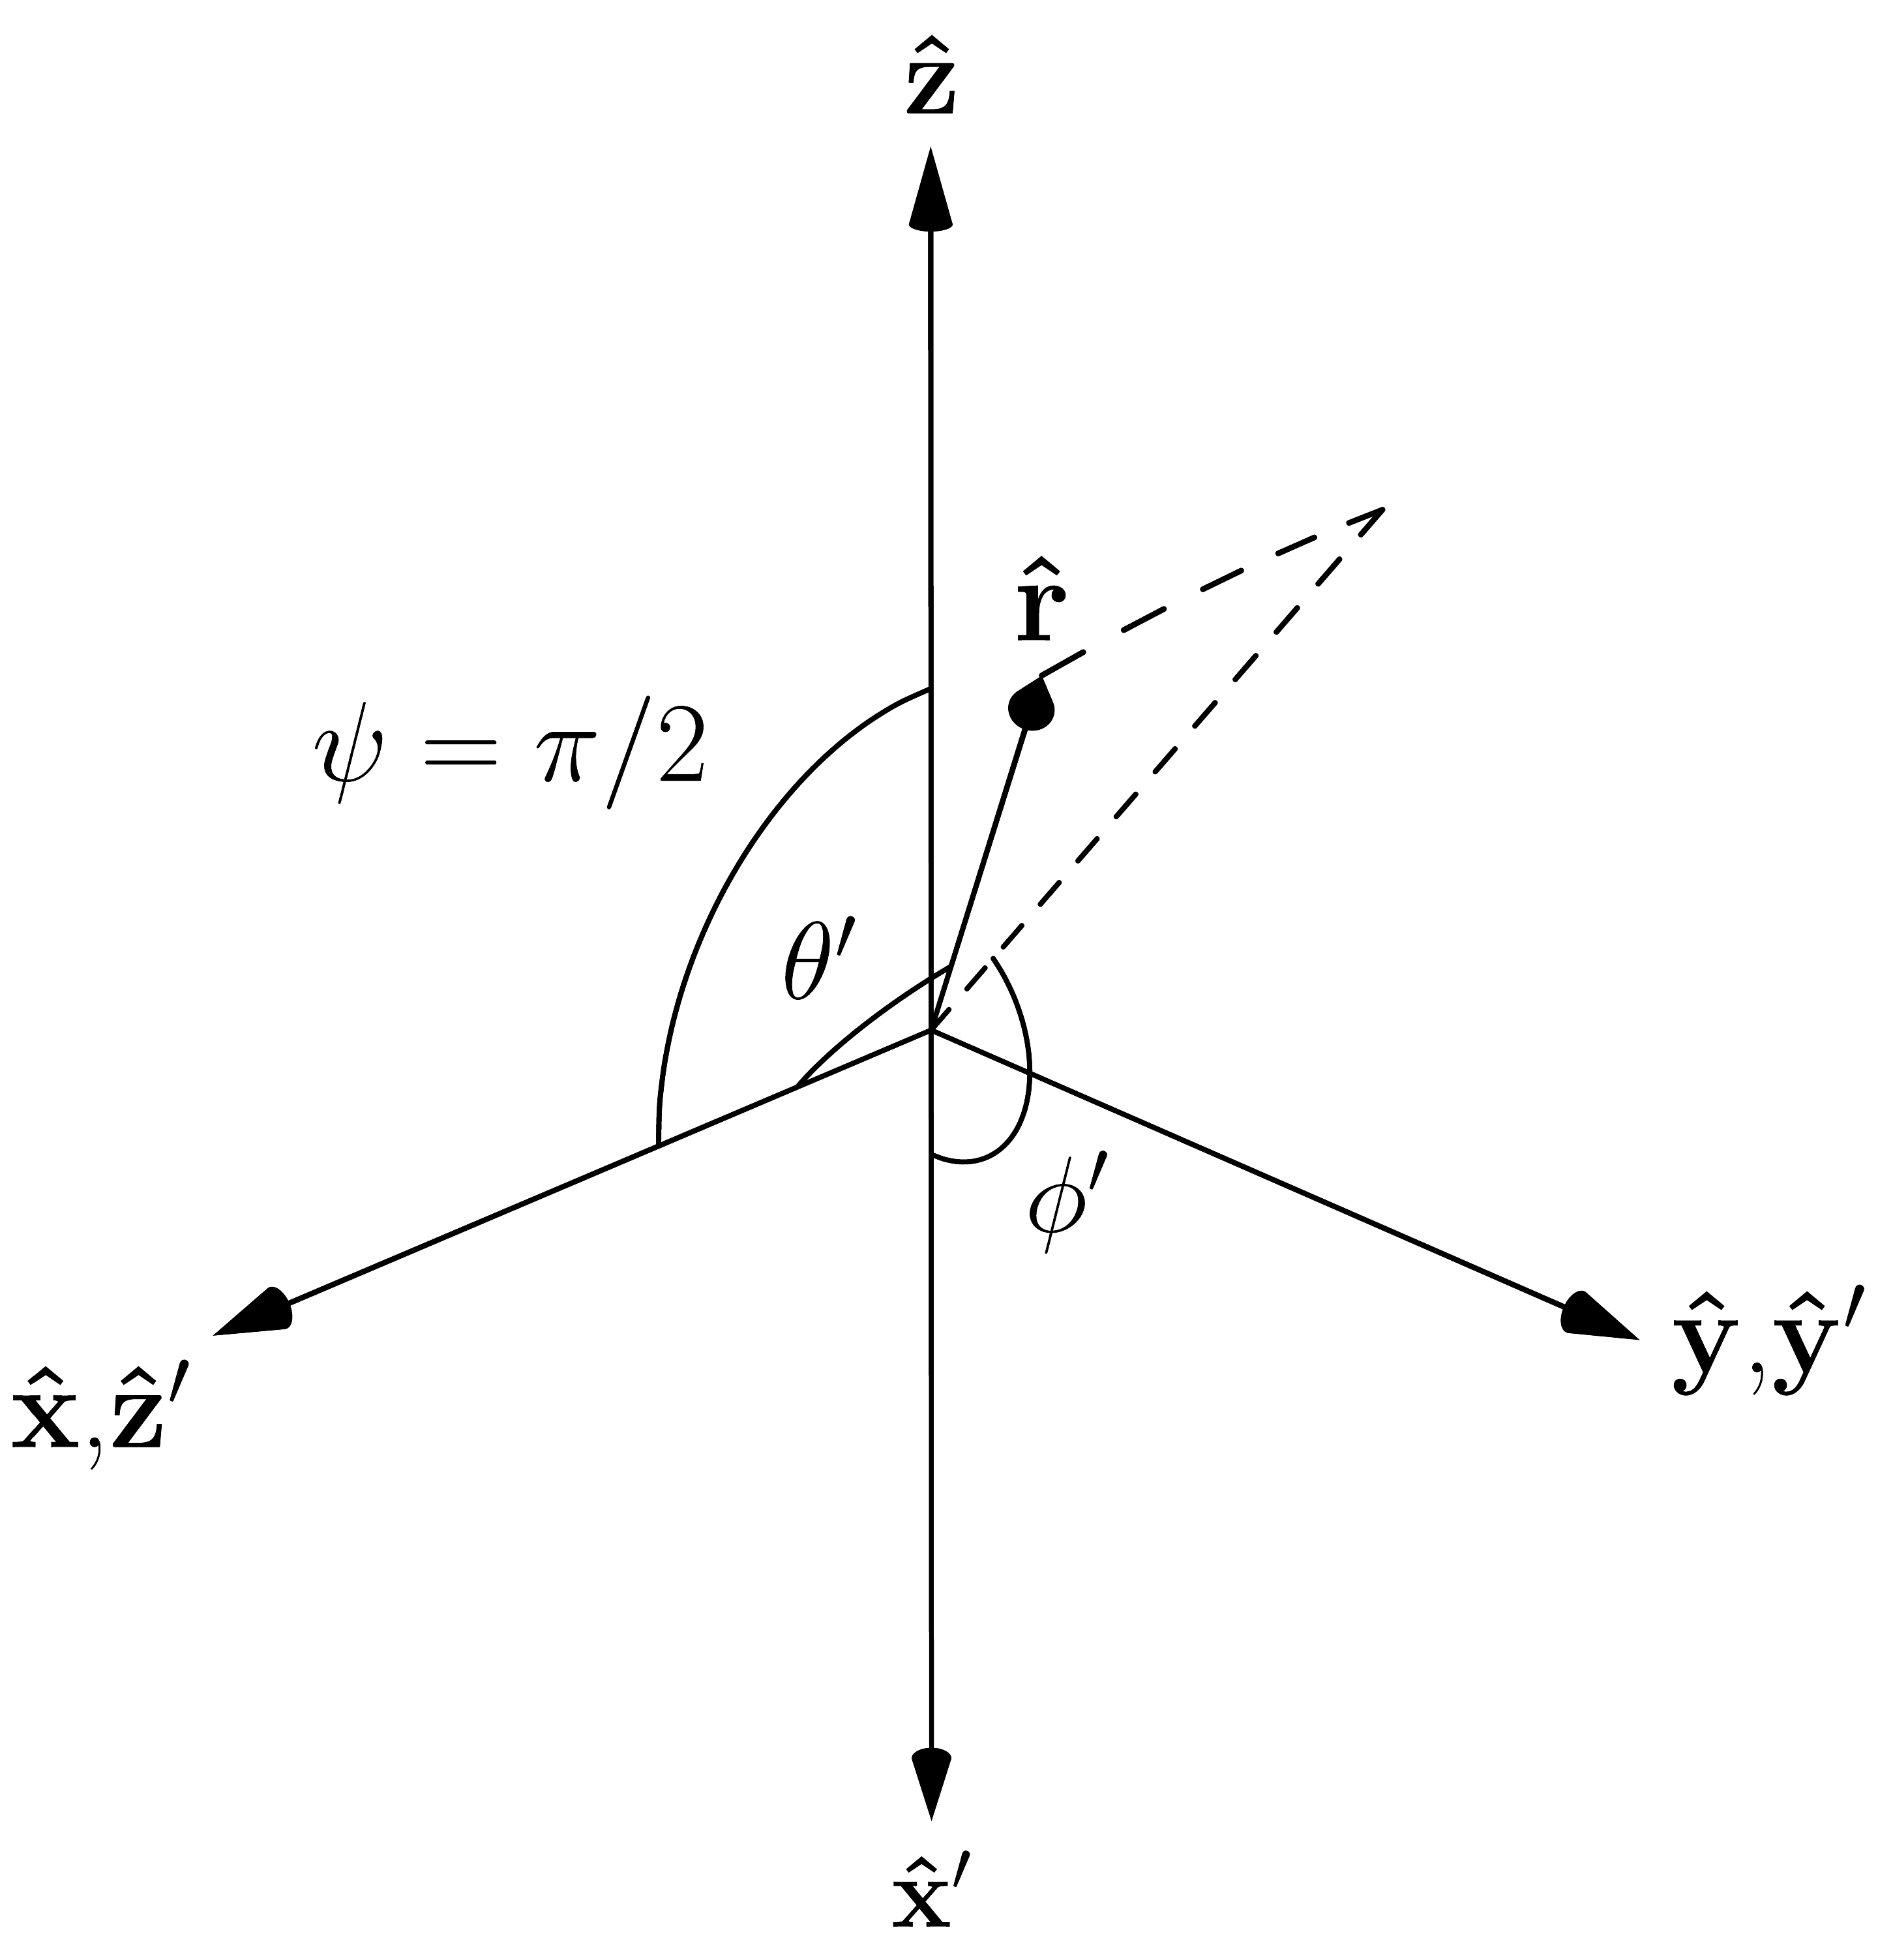
\includegraphics[width = 1.0\textwidth]{../figures/frame_c.pdf}
   \caption{Orthogonal spherical coordinates}
   \label{fig:frames_c}
 \end{subfigure}%
 \caption{Possible spherical coordinate definitions.}
 \label{fig:frames}
\end{figure*}

\section{Relating Spherical Coordinates In Two Oblique Frames}
First, we expand a single unit vector $\mh{r}$ in two different coordinate systems
\begin{align}
  \mh{r} = x\mh{x} + y\mh{y} + z\mh{z} &= x'\mh{x}' + y'\mh{y}' + z'\mh{z}'.
\intertext{Next, we rewrite the vector in spherical coordinates}
  \mh{r} = \cos\phi\sin\theta\mh{x} + \sin\phi\sin\theta\mh{y} + \cos\theta\mh{z} &= \cos\phi'\sin\theta'\mh{x}' + \sin\phi'\sin\theta'\mh{y}' + \cos\theta'\mh{z}'.\label{eq:sphere}
\end{align}
Finally, we relate the coordinate systems. We will only consider coordinate
systems that are related by a right handed rotation by angle $\psi$ about the
$\mh{y}$ axis, so the coordinate systems are related by
\begin{subequations}
\begin{align}
  \mh{x} &= \cos\psi\mh{x}' +\sin\psi\mh{z}'\\
  \mh{y} &= \mh{y}'\\
  \mh{z} &= -\sin\psi\mh{x}' + \cos\psi\mh{z}'.
 \end{align}\label{eq:coords}
\end{subequations}%
Plugging equation \ref{eq:coords} into equation \ref{eq:sphere} and equating
each component gives
\begin{subequations}
  \begin{align}
    \cos\psi\cos\phi\sin\phi - \sin\psi\cos\theta\label{eq:preva} &=\cos\phi'\sin\theta'\\
     \sin\phi\sin\theta&=\sin\phi'\sin\theta' \label{eq:prevb}\\
    \sin\psi\cos\phi\sin\theta + \cos\psi\cos\theta&=\cos\theta' .\label{eq:prevc}
  \end{align}
\end{subequations}
Solving for $\theta'$ and $\phi'$ in terms of $\theta$, $\phi$, and $\psi$ gives
\begin{subequations}
\begin{align}
  \theta' &= \arccos\left(\sin\psi\cos\phi\sin\theta + \cos\psi\cos\theta\right)\label{eq:thetap}\\
  \phi' &= \arccos\left(\frac{\cos\psi\cos\phi\sin\phi - \sin\psi\cos\theta}{\sqrt{1 - (\sin\psi\cos\phi\sin\theta + \cos\psi\cos\theta)^2}}\right).\label{eq:phip}
\end{align}\label{eq:solution}% 
\end{subequations}
Equation \ref{eq:thetap} follows directly from equation \ref{eq:prevc}. Equation
\ref{eq:phip} follows from plugging equation \ref{eq:thetap} into equation \ref{eq:prevc} and using the identity $\sin(\arccos(x)) = \sqrt{1 - x^2}$.

The inverse equations can be found by the substituting $\psi \rightarrow -\psi$:
\begin{subequations}
\begin{align}
  \theta &= \arccos\left(-\sin\psi\cos\phi'\sin\theta' + \cos\psi\cos\theta'\right)\\
  \phi &= \arccos\left(\frac{\cos\psi\cos\phi'\sin\phi' + \sin\psi\cos\theta'}{\sqrt{1 - (\sin\psi\cos\phi'\sin\theta' + \cos\psi\cos\theta')^2}}\right).
\end{align}\label{eq:solutionp}% 
\end{subequations}


\section{Relating Spherical Coordinates In Two Orthogonal Frames}
Setting $\psi = \pi/2$ in equation \ref{eq:solution} gives
\begin{subequations}
  \begin{align}
  \theta' &= \arccos\left(\cos\phi\sin\theta\right)\\
  \phi' &= \arccos\left(\frac{-\cos\theta}{\sqrt{1 - \cos^2\phi\sin^2\theta}}\right).
\end{align} \label{eq:solution2}%
\end{subequations}
The inverse equations are
\begin{subequations}
\begin{align}
  \theta &= \arccos\left(-\cos\phi'\sin\theta'\right)\\
  \phi &= \arccos\left(\frac{\cos\theta'}{\sqrt{1 - \cos^2\phi'\sin^2\theta'}}\right).
\end{align} \label{eq:solution2p}% 
\end{subequations}
We'll test these equations with $\theta = \pi/4$ and $\phi=\pi/3$ as illustrated in
Figure \ref{fig:frames_a}. Plugging into equation \ref{eq:solution2} gives
\begin{subequations}
\begin{align}
  \theta' &= \arccos\left(\cos(\pi/3)\sin(\pi/4)\right) = 1.21 = 69.0^{\circ}\\
  \phi' &= \arccos\left(\frac{-\cos(\pi/4)}{\sqrt{1 - \cos^2(\pi/3)\sin^2(\pi/4)}}\right) = 2.43 = 139.1^{\circ}
\end{align}\label{eq:check1}%
\end{subequations}
which is consistent with Figure \ref{fig:frames_c}. We'll test the inverse equation as
well. Plugging equation \ref{eq:check1} into equation \ref{eq:solution2p} gives
\begin{subequations}
\begin{align}
  \theta &= \arccos\left(-\cos(2.43)\sin(1.21)\right) = \pi/4\\
  \phi &= \arccos\left(\frac{\cos(1.21)}{\sqrt{1 - \cos^2(2.43)\sin^2(1.21)}}\right) = \pi/3
\end{align}\label{eq:check1}% 
\end{subequations}
as expected. 


\section{Discussion}
Equations \ref{eq:solution2} and \ref{eq:solution2p} will be useful for
analyzing data collected with the polarization diSPIM. If we measure $\theta$
and $\phi$ in both views with the optical axis along the $\mh{z}$ axis, then we
can use the equations \ref{eq:solution2} and \ref{eq:solution2p} to convert the
measurements to the same coordinate system. Note that these equations will only
work if the $\mh{y}$ axis is defined as the normal to the plane containing the
optical axes.
\end{document}

